\documentclass[emulatestandardclasses]{scrartcl}
\usepackage{graphicx}
\usepackage{color}
\usepackage[ngerman]{babel}
\usepackage{hyperref}
\usepackage{fullpage}
\usepackage{calc} 
\usepackage{enumitem}
\usepackage{titlesec}
\newcommand{\todo}[1]{\textcolor{red}{TODO: #1}\PackageWarning{TODO:}{#1!}}
\date{\vspace{-3ex}}
\begin{document}

\title{
	\includegraphics*[width=0.75\textwidth]{images/hu_logo.png}\\
	\vspace{24pt}
	Einf"uhrung in die Philosophie}
\subtitle{Vorlesung WS 16/17\\
          Prof. Dr. Thomas Schmidt\\
          Philosophisches Institut I \\ 
          Humboldt Universit"at zu Berlin}
\author{Lennard Wolf\\
        \small{\href{mailto:lennard.wolf@student.hu-berlin.de}{lennard.wolf@student.hu-berlin.de}}}
\maketitle
\begin{abstract}

Die Vorlesung bietet eine Einf"uhrung in f"ur die Philosophie charakteristische Fragestellungen, Denkweisen und Theorieans"atze sowie in Begriffe, deren Kenntnis zum philosophischen Handwerkszeug geh"ort. Im Vordergrund steht die exemplarische Auseinandersetzung mit ausgew"ahlten philosophischen Sachproblemen aus verschiedenen Teilgebieten der Philosophie.

\end{abstract}
\newpage

\tableofcontents
\listoffigures
\newpage


\section{Einf"uhrung / Logische Prop"adeutik\\(20.10.16)}

\subsection{Einf"uhrung}
\subsubsection{Was ist Philosophie?}

\begin{itemize}
  \item Professoren sind sehr uneinig "uber diese Frage
  \item Kein \emph{Laberfach}, sondern ''Verstehen, was die Welt im Inneren zusammenh"alt'' (Faust)
  \item Sie ist der Ursprung aller Einzelwissenschaften -- bleibt nichts "ubrig mehr nach der Zergliederung?
  \item Wissenschaft ist h"aufig nur \emph{Hingucken}, Philosophie ist zus"atzlich \emph{Nachdenken}\\(''I sit down and think.'' $\rightarrow$ \emph{armchair philosophy})
  \item \emph{Willensfreiheit vs. Determinismus} ist klassisch philosophische Fragestellung
\end{itemize}

\subsubsection{Willensfreiheit vs. Determinismus}

\begin{itemize}
  \item Empirie zeigt, dass alles deterministisch verl"auft
  \item Ob Willensfreiheit mit diesem Determinismus vereinbar ist ist keine empirische Frage (Status quo der Philosophen ist, dass es vereinbar ist)
\end{itemize}

\subsubsection{Philosophische Fragestellungen / Teilgebiete}

\begin{itemize}
  \item \emph{Ontologie}: Was ist die Struktur der Realit"at / Was gibt es?
  \item \emph{Erkenntnistheorie}: Was ist Wissen? Was f"ur Arten dessen gibt es?
  \item \emph{Metaphysik}: Was ist Wahrheit? (???)
  \item \emph{Normative / Werttheoretische Fragen}: Was ist ein gutes Leben? Wie soll man handeln?
\end{itemize}

\subsubsection{Philosophie und ihre Geschichte}

\begin{itemize}
  \item Anders als bei anderen Wissenschaften: Klassische philosophische Theorien sind auch heute noch ernst zu nehmen
  \item Historisches Bewusstsein ist in der Philosophie essenziell (\emph{elder contemporary view}, "altere Zeitgenossen wie Aristoteles sollte man sch"atzen k"onnen)
  \item Forschung in der Geschichte der Philosophie ist aber eher unerheblich, es geht vielmehr um tats"achliche Sachfragen
\end{itemize}

\subsection{Konzeption der Vorlesung}

\subsubsection{Was die Vorlesung bietet}

\begin{itemize}
  \item Eine Art philosophisches Glossar
  \item Teilgebiete werden durch Problemstellungen n"aher gebracht
\end{itemize}


\subsubsection{Was die Vorlesung nicht bietet}

\begin{itemize}
  \item {\color{red}(???)}
\end{itemize}

\subsubsection{Was die Vorlesung von uns erwartet}

\begin{itemize}
  \item \emph{Meinung haben ist leicht, Meinung begr"unden ist schwer!}
  \item Aktives Nachdenken in der Vorlesung!
\end{itemize}

\subsection{Logische Prop"adeutik: Was ist ein gutes Argument?}

\subsubsection{Was sind Argumente?}

Begr"undungen f"ur Meinungen / Sind Antworten auf \emph{Warum}-Fragen zu Meinungen

\subsubsection{Begr"undungen vs. Erkl"arungen}

Begr"undungen sind gefragt, wenn die Konklusion fraglich ist, w"ahrend bei Erkl"arungen der Wahrhaftigkeit der Konklusion außer Frage steht


\subsubsection{Struktur von Argumenten}
\textbf{Normalform:}  Pr"amissen (P1 -- Pn) $\rightarrow$ Konklusion (K)


\subsubsection{Was ist ein gutes Argument?}

???

\subsection{Tutorium}

\textbf{-- abwesend --}
\newline

Es m"ussen 3 Essays (5 - 6 Seiten) abgegeben werden um das Tutorium zu bestehen (am besten um Weihnachten rum schreiben). Ganz klare Fragestellung die mit den Fertigkeiten aus den Tutorien relativ einfach gel"ost werden k"onnen.


\newpage

\section{Metaphysik I: Was gibt es?\\(27.10.16)}

\subsection{Was ist Metaphysik?}


\subsubsection{Das traditionelle Verständnis von Metaphysik}


\subsubsection{Metaphysik und Ontologie, allgemeine und spezielle Metaphysik}


\subsubsection{Metaphysik in der Philosophie der Gegenwart}



\subsubsection{Metaphysikkritik}


\subsection{Was gibt es? -- Quine über ontologische Verpflichtungen}


\subsubsection{Metaphysik der Einf"uhrungs-Vorlesung}



\subsection{Fallbeispiel: Gibt es moralische Tatsachen (bzw. Werte)?}

\subsection{Tutorium}
\subsubsection{Tips f"ur guten Stil bei Hausaufgaben}

\begin{itemize}
  \item keine Schulmeisterprosen / keine UGS
  \item Pr"apositionen
  \item Klarheit, Genauigkeit; Sorgfalt; scharfe Begriffe vorziehen
  \item Konjunktiv I f"ur die indirekte Wiedergabe (Konjunktiv II dr"uckt Zweifel aus)
  \item Verbklammern m"oglichst klein halten
  \item kurze, pr"agnante S"atze; m"oglichst wenige Nebens"atze
  \item Konjunktionen beachten
\end{itemize}

\subsubsection{Wichtige Terme}

\begin{description}[leftmargin=!,labelwidth=\widthof{\bfseries Ontologische Verpflichtung (Quine)}]
  \item[Metaphysik] Fragen nach der fundamentalen Struktur der Realit"at
  \item[Tatsachen] \emph{Es ist der Fall, dass...}
  \item[Entit"at]   {\color{red}(???)}
  \item[Ontologische Verpflichtung (Quine)] Alles was in der besten Theorie... Wir m"ussen wir als existierend annehmen {\color{red}(???)}
  \item[Gute Theorie] Theorie ist gut wenn sie prognostische Kraft hat und Ockhams Razor erf"ullt
  \item[Deontische Indikatoren] \emph{sollte}, \emph{es ist ver/geboten, dass}, ...
  \item[Pr"amissenindikatoren] \emph{weil}, \emph{wegen}, \emph{da}...
  \item[Konklusionsindikatoren] \emph{also}, \emph{somit}, \emph{daher}, \emph{demnach}, \emph{demzufolge}
\end{description}

\textbf{Zu lesen: }

\emph{"Uberwindung der Metaphysik durch die logische Analyse der Sprache} -- Rudolf Carnap

\emph{Handwerk des Philosophischen Schreibens} -- Philip H"uhl ($\approx$ 30 Seiten)

Erste 20 - 30 Seiten des Dudens

\section{Metaphysik II: Sind Freiheit und Determinismus vereinbar?\\(02.11.16)}

\emph{Metaphysika Specialis}

\subsection{Auftakt}

\textbf{Determinismus:} Vergangenheit + Naturgesetze = Zukunft $\rightarrow$ Alles steht fest


\begin{itemize}
  \item
\end{itemize}


\subsection{Willensfreiheit: Verschiedene Positionen}

\subsubsection{Inkompatibilismus}

\subsubsection{Kompatibilismus}

\subsubsection{Relevanz der Frage nach Willens- und Handlungsfreiheit}

\subsection{Die inkompatibilistische Herausforderung}

"Odipus t"otete einen Mann (der sein Vater war, ohne dass er es wusste) an der Weggabelung. Er hat aus freien St"ucken einen fremden Mann get"otet (Daf"ur ist er verantwortlich), jedoch nicht seinen Vater (Daf"ur kann er nicht verantwortlich gemacht werden). Zur Kontrolle geh"ort, anders handeln zu k"onnen.

\subsection{Kann die inkompatibilistische Herausforderung zur"uckgewiesen werden?}
Wenn Inkompatibilismus wahr ist: 
\begin{enumerate}
  \item Wir m"ussten allen Menschen gegen"uber immer eine \emph{Objective Attitude} einnehmen.
  \item ..
  \item ..
\end{enumerate}

Frankfurt

Fahrschule, man muss fahren, man tut alles richtig. H"atte man falsch gehandelt
\subsection{Wichtige Terme}

\begin{description}[leftmargin=!,labelwidth=\widthof{\bfseries Moralische Verantwortlichke}]
  \item[Kontrolle] {\color{red}(???)}
  \item[Moralische Verantwortlichkeit] {\color{red}(???)}
  \item[Objective Attitude] {\color{red}(???)}
  \item["Aquivokationsfehlschlu\ss] Vermischen von Begriffen in den Pr"amissen
  \item[Intention] Absicht  
\end{description}

\subsection{Tutorium}


\begin{itemize}
  \item Korrekte Grammatik und Rechtschreibung (!!!)
  \item DIN Regeln Latex?
  \item Stilregeln:
  \item Indirekte Wiedergebe von Rede: Konjunktiv 2 zweifelt an, Konjunktiv 1 ist neutral | Ausnahme: \emph{Er sagt, dass andere Welten existieren w"urden.}
  \item \emph{Laut}, \emph{Zufolge}, \emph{Nach}
  \item Anscheinend (Beste Theorie nach gegebenem Wissen), Scheinbar (Zweifelnd)
  \item Bei Rekonstruktion immer erst die Konklusion klar machen
\end{itemize}

\section{Erkenntnistheorie I: Was ist Wissen?\\(17.11.16)}

\subsection{Auftakt}

\begin{description}[leftmargin=!,labelwidth=\widthof{\bfseries Propositionelles Wissen}]
  \item[Erkenntnis] Synonym zu Wissen
  \item[Erkenntnistheorie] Philosophisches Nachdenken \emph{"uber} Wissen (Nicht \emph{Erweitern} von Wissen) | Fragen nach dem \emph{Wesen von Wissen}: Was haben die Dinge gemein, die sie zu Wissen macht? Was kann man (prinzipiell) wissen? Was ist der Unterschied zu Nichtwissen? | In der Neuzeit in Vordergrund ger"uckt, in der Antike mehr Metaphysisches, Ontologisches; denn: Wie k"onnen wir "uber Ontologie reden wenn wir nicht wissen, was wir wissen k"onnen? 
  \item[Erfahrungswissen] Form des Satzes "`Sie wei"s, wie man Fahrrad f"ahrt."' ist \emph{Wissen Wie}, Erfahrungswissen | Ist das "uberhaupt \emph{Wissen}?
  \item[Propositionelles Wissen] Form des Satzes "`Er wei"s, dass unser Sonnensystem 8 Planeten hat."' ist \\"`$S$ wei"s, dass $p$."' | Kernthema der Erkenntnistheorie
  \item[Frage nach dem Wesen] "`Was ist das Wesen von $x$?"' $\rightarrow$ "`Etwas ist ein $x$ \emph{genau dann wenn} f"ur es $1$, $2$,..., $n$ der Fall ist."' | Hat ein Tisch Beine? -- Ein Tisch ist ein Tisch wenn er Beine hat und man was drauf stellen kann. Aber das gilt f"ur uns ja auch. | Eine Antwort setzt nicht vorraus dass es das gibt! (Beispiel Einhorn) Wenn man also nach dem Wesen des Wissens fragt macht man noch keine Existenzaussage.
\end{description}

\subsection{Klassische Wissenskonzeption}

\textbf{Notwendige Bedingungen f"ur Wissen nach der klassischen Wissenskonzeption}

\begin{description}[leftmargin=!,labelwidth=\widthof{\bfseries $(1)$ Rechtfertigungi}]
  \item[$(1)$ Meinung] "`$S$ ist der Meinung, dass $p$."' im Sinne von \emph{vermuten} | Ist Notwendige Bedingung denn wenn $S$ nicht von $p$ "uberzeugt ist, w"urde $S$ auch nicht sagen, dass sie wei"s, dass $p$.
  \item[$(2)$ Wahrheit] "`$p$ ist wahr."' | Ist notwendig, da "`$S$ wei"s, dass $p$, aber $p$ ist falsch."' sinnlos ist. (Beispiel: "`Fr"uher wussten die Leute, dass die Erde eine Scheibe ist."' w"are nur sinnig, wenn die Erde auch fr"uher eine Scheibe war.)
  \item[$(3)$ Rechtfertigung] "`$S$ ist in der Meinung, dass $p$, gerechtfertigt."' | N"otig denn Meinung und Wahrheit sind noch nicht hinreichend, denn Zufallstreffer etc. sind ja kein \emph{Wissen}. 
\end{description}

Die Bedingungen $(1)$, $(2)$ und $(3)$ f"ur den \emph{Justfied True Belief} (Wahre, gerechtfertigte Meinung) sind gemeinsam hinreichend. Das hei"st:

"`$S$ wei"s, dass $p$."' \hspace{1mm} $\Leftrightarrow$ \hspace{2mm}"`$S$ ist der Meinung, dass $p$."' $\wedge$

\hspace{35mm} "`$p$ ist wahr."' $\wedge$

\hspace{36mm}"`$S$ ist in der Meinung, dass $p$, gerechtfertigt."'

\subsection{Der Einwand von Edmund Gettier}

\textbf{Gettiers Argument} (aus \emph{Is Justfied True Belief Knowledge?})

\begin{description}[leftmargin=!,labelwidth=\widthof{\bfseries Gegenbeispiel 2}]
  \item[Pr"amisse 1] Rechtfertigung impliziert nicht Wahrheit; $(2)$ und $(3)$ sind unabh"angig
  \item[Pr"amisse 2] Wenn $S$ in der Meinung, dass $p$, gerechtfertigt ist, und wenn $q$ aus $p$ logisch folgt, und wenn $S$ aufgrund dieser Tatsache die Meinung, dass $q$, annimmt, dann ist $S$ auch in der Meinung, dass $q$, gerechtfertigt.
  \item[Gegenbeispiel 1] (\emph{Er wurd der `gegettiert'.})
  \item[Gegenbeispiel 2] 
\end{description}

\subsection{Reaktionen auf Gettiers Einwand}

Einfach L"osungen scheint es nicht zu geben.
\begin{itemize}
  \item Dass Rechtfertigung Wahrheit impliziert schraubt Anforderungen an Wissen zu hoch ???
  \item 
\end{itemize}

\textbf{L"osungsstrategien}

Einfach L"osungen scheint es nicht zu geben.
\begin{itemize}
  \item Gettierologie: Die Suche nach der vierten Bedingung
  \item Kausale Wissenskonzeption: 
\end{itemize}


\subsection{Tutorium}

\begin{itemize}
  \item Immer mit Fu"snoten zitieren und Fu"snote dann \emph{nach} Punkt bzw. Semikolon
  \item Ebenda | a.a.O; S. x
  \item \emph{Rabulistik}: Wortklauberei (Schopenhauer)
  \item Hausarbeitsgr"o"sen: Hausarbeit Proseminar 25 000 Zeichen bzw. 10 000 Zeichen (in Wahlfrei II) | Hausarbeit Hauptseminar 35 000 Zeichen
  \item Essay f"ur Einf"urhungsseminar: Winziger Ausschnitt (Textsorte nennen) z.B. Kant, Wittgenstein $\rightarrow$ wo man gut interpretieren kann |
  \item Hausarbeit: Einleitung: Pr"azise und ad"aquat Thema einschr"anken und exaktes Vorgehen beschreiben. (Auch: Wo kommt das her?); \emph{Was wir sagen werden}; Hauptteil: Was wir sagen Schluss: Was wir gesagt haben.
  \item Exerpieren: Knowledge Maps
\end{itemize}


\section{Erkenntnistheorie II: Was k"onnen wir wissen?\\(23.11.16)}

\subsection{Arten von Wissen: M"ogliche Kandidaten}
\textbf{Unterschiedliche Inhalte des Wissens}\\
Wissen "uber \emph{konkrete Inhalte} | Wissen "uber \emph{Naturgesetze} | Wissen um \emph{sprachliche Bedeutung} | \emph{mathematisches} Wissen | \emph{moralisches} Wissen

\hspace{3mm}$\rightarrow$ Kann in all diesen Bereichen die Rede von Wahrheit sein?
\newline

\noindent\textbf{Rechtfertigungen f"ur Wissens}\\
Unmittelbare Erfahrung | mittelbare Erfahrung ("`vom H"orensagen"' -- Naturgesetze per Induktion gerechtfertigt?) | Ohne Erfahrung (z.B. Deduktiv)

\begin{description}[leftmargin=!,labelwidth=\widthof{\bfseries A posteriorisches Wissen}]
  \item[A priorisches Wissen] Wissen das keine Erfahrung ben"otigt (\emph{a priori} gerechtfertigte Meinung, doch wann ist solches Wissen interessant?)
  \item[A posteriorisches Wissen] Empirisches Wissen (Mit Erfahrung gerechtfertigte Meinung)
  \item[Analytisches Urteil] Wenn das Pr"adikat in dem Subjekt schon versteckt vorkommt.
  \item[Synthetisches Urteil] Wenn das Pr"adikat in dem Subjekt nicht versteckt vorkommt.
\end{description}
%\vspace{3mm}
\noindent\textbf{Synthetisches Wissen \emph{a priori}}\\

\begin{center}
Philosophie scheint nur sinnvoll zu sein, wenn es synthetisches Wissen \emph{a priori} gibt.
\end{center}

M"unchhausen Trilemma: Wenn ich $p$ wei"s, dann muss ich in $p$ gerechtfertigt sein. In einer Argumentation, in der $p$ die Konklusion ist, m"uss ich in den Pr"amissen auch gerechtfertigt sein. Doch ich muss auch in deren Pr"amissen gerechtfertigt sein und in deren etc. etc.\\
Drei \emph{H"orner}: Unendlicher Regress; Muss irgendwo dogmatisch abbrechen; Zirkularit"at

$\rightarrow$ \emph{Foundationalism}: Ich breche bei der sinnlichen Erfahrung ab.

\begin{enumerate}
	\item Frage 2: Was \textbf{k"onnen} wir wissen?
	\item Arten von Wissen: m"ogliche Kandidaten
	\item apriorisches vs. aposteriorisches Wissen
	\item Gibt es apriorisches Wissen?
	\item Gibt es empirisches Wissen?
\end{enumerate}
\subsection{Was k"onnen wir wissen?}
Die Frage setzt \textbf{keine} antiskeptische Haltung vorraus.
\subsection{Arten von Wissen: m"ogliche Kandidaten}
Kategorisierung anhand des \textbf{Inhalts}:
\begin{enumerate}
	\item Tatsachenwissen
	\item Naturgesetze
	\item sprachliches Wissen(lies:\textit{begrifflich})
	\item mathematisches Wissen
	\item moralisches Wissen
	\item Wissen um Konventionen(Beitrag)
\end{enumerate}
Kategorisierung anhand der \textbf{Rechtfertigung}:
\begin{enumerate}
	\item Wissen aufgrund von unmittelbarer Erfahrung
	\item Wissen das mittelbar der Erfahrung entstammt["H"orensagen"]
	\item Wissen das nicht der Erfahrung entstammt
\end{enumerate}
\subsection{Apriorisches vs. aposteriorisches Wissen}
Referenz für Unterscheidung: Kant in KdrV
\\ \\
Aposteriorisches Wissen:Kann nur aus Erfahrung gewonnen worden
\\ \\
Apriorisches Wissen:
\begin{itemize}
	\item[i]von der Erfahrung unabhängiges Wissen(nicht zeitlich gemeint)
	\item[ii] dies heisst nichts dass es unm"oglich ist es a posteriori zu wissen
\end{itemize}
\subsection{Gibt es a priorisches Wissen}
Analytische vs. synthetische Urteile:
\begin{itemize}
	\item[i] Sch"arfer: Gibt es \textit{informatives} apriorisches Wissen ?
	\item[ii] Was heisst informativ: Kant: synthetisch/analytisch
	\item[iii] Allgemeiner: Wahrheiten sind analytisch wenn:\par p $\wedge$ Wahrheit von P ist nur mit Sprache und Logik erkennbar\\
\end{itemize}
\subsection{Allgemeines}
Motivation für Kant: Zwiespalt zwischen Faszination für Naturwissenschaften und spekulativen metaphysischen Debatten("Kampfplatz endloser Streitigkeit")
\section{Tutorium am 28.11.16\\Erkenntnistheorie}
Aufarbeitung der Vorlesung
\subsection{Vorlesung}
Bereiche der Erkenntnistheorie\\
Besprechung der Gettier Fälle

	\subsubsection {Was ist Wissen?} \begin{enumerate}
	\item Propositionales Wissen (Wissen dass...)
	\item Handlungswissen(Wissen wie)
	
	\item \textbf{Wichtig}: Trennung Wissensanspruch/tatsächliches Wissen
	\item Klassische Wissensdefinition(JTB)
	 \begin{enumerate}
	 	\item Ich bin der \emph{Überzeugung} dass
	 	\item Ich bin darin \emph{gerechtfertigt}
	 	\item Diese Überzeugung ist \emph{wahr}
	 \end{enumerate}
	 \end{enumerate}
	
	\subsubsection{Was k"onnen wir Wissen?} 
	Erste Trennung: Über die Aussenwelt/Über uns selbst
	\begin{table}[hbt]
  \begin{tabular}{l|c|c|r}
    &analytisch &synthetisch \\
    \hline
    &1 & (nach Kant) 1 \\
    &0 &1
  \end{tabular}
  %\caption{}
\end{table}


\subsection{Allgemeines}
\begin{enumerate}
\item Proposition= Inhalt eines Aussagesatzes
\item JTB ist eine reduktive Definition. Begriffe werden zerlegt bis mensch bei Grundbegriffen angelangt ist. Oft wird dies für die einzige Art der Begrifssanalyse gehalten.  Lektüre zur Gegenposition: Wittgenstein-Philosophische Untersuchungen und Strawson-Bodies 
\end{enumerate}


\section{Wissenschaftstheorie: Wie funktioniert (Natur-) Wissenschaft?\\(01.12.16)}

\subsection{Was ist Wissenschaftstheorie}

\begin{description}[leftmargin=!,labelwidth=\widthof{\bfseries Poppers Falsifikationismus}]
  \item[Wissenschaftstheorie] (auch Wissenschaftsphilosophie)
  \item[Induktivismus] Wissenschaft beginnt mit Beobachtung, man sammelt immer mehr ebendieser und schlie"st aus diesen allgemeine Gesetze/Theorien (Von den logischen Empiristen aus dem Wiener Zirkel, \emph{Protokollsatzsprache}) | Probleme: aus endlichen Beobachtungen folgen keine Allaussagen (Induktionsproblem); Beobachten in der Wissenschaft ist meist theoriegeleitet (Normativ)
  \item[Poppers Falsifikationismus] Wissenschaft started mit Theorien (Vermutungen), diese Leiten zu Beobachtungen an, mit welchen man versucht, die Theorie zu falsifizieren [auch \emph{Kritischer Rationalismus}] (Normativ)
  \item[Positivismusstreit] Streit zwischen Frankfurter Schule und Logischen Empiristen | Adorno etc: Holismus, keine Gesetze
  \item[Feyerabend] Anything goes. (Deskriptiv)
  \item[Kuhn] Paradigmen und Analogien. (Deskriptiv)
\end{description}

\subsection{Wissenschaftsphilosophie vs. Geschichte}

Was ist die Grundthese des Substanzdualismus?
Mentales und Nichtmentales sind real verschieden.

Was spricht f"ur den Interaktionistischen Dualismus?

Was ist die Grundthese des Parallelismus?

Dass sich mentale und nichtmentale Ereignisse zeitlich parallel, aber kausal voneinander unabh"angig abspielen.

Was ist die Grundthese des Epiph"anomenalismus?
Eigenschaftsdualismus


Was ist die Grundthese des Funktionalismus?



\section{Sprachphilosophie I: Was ist sprachliche Bedeutung?\\(08.12.16)}

Analytische Philosophie nach Russell: What do you mean? How do you know?

\newpage
\section{"Uber den Professor}
Prof. Mustermann ist..


%\begin{figure}[h]
%	\centering
%	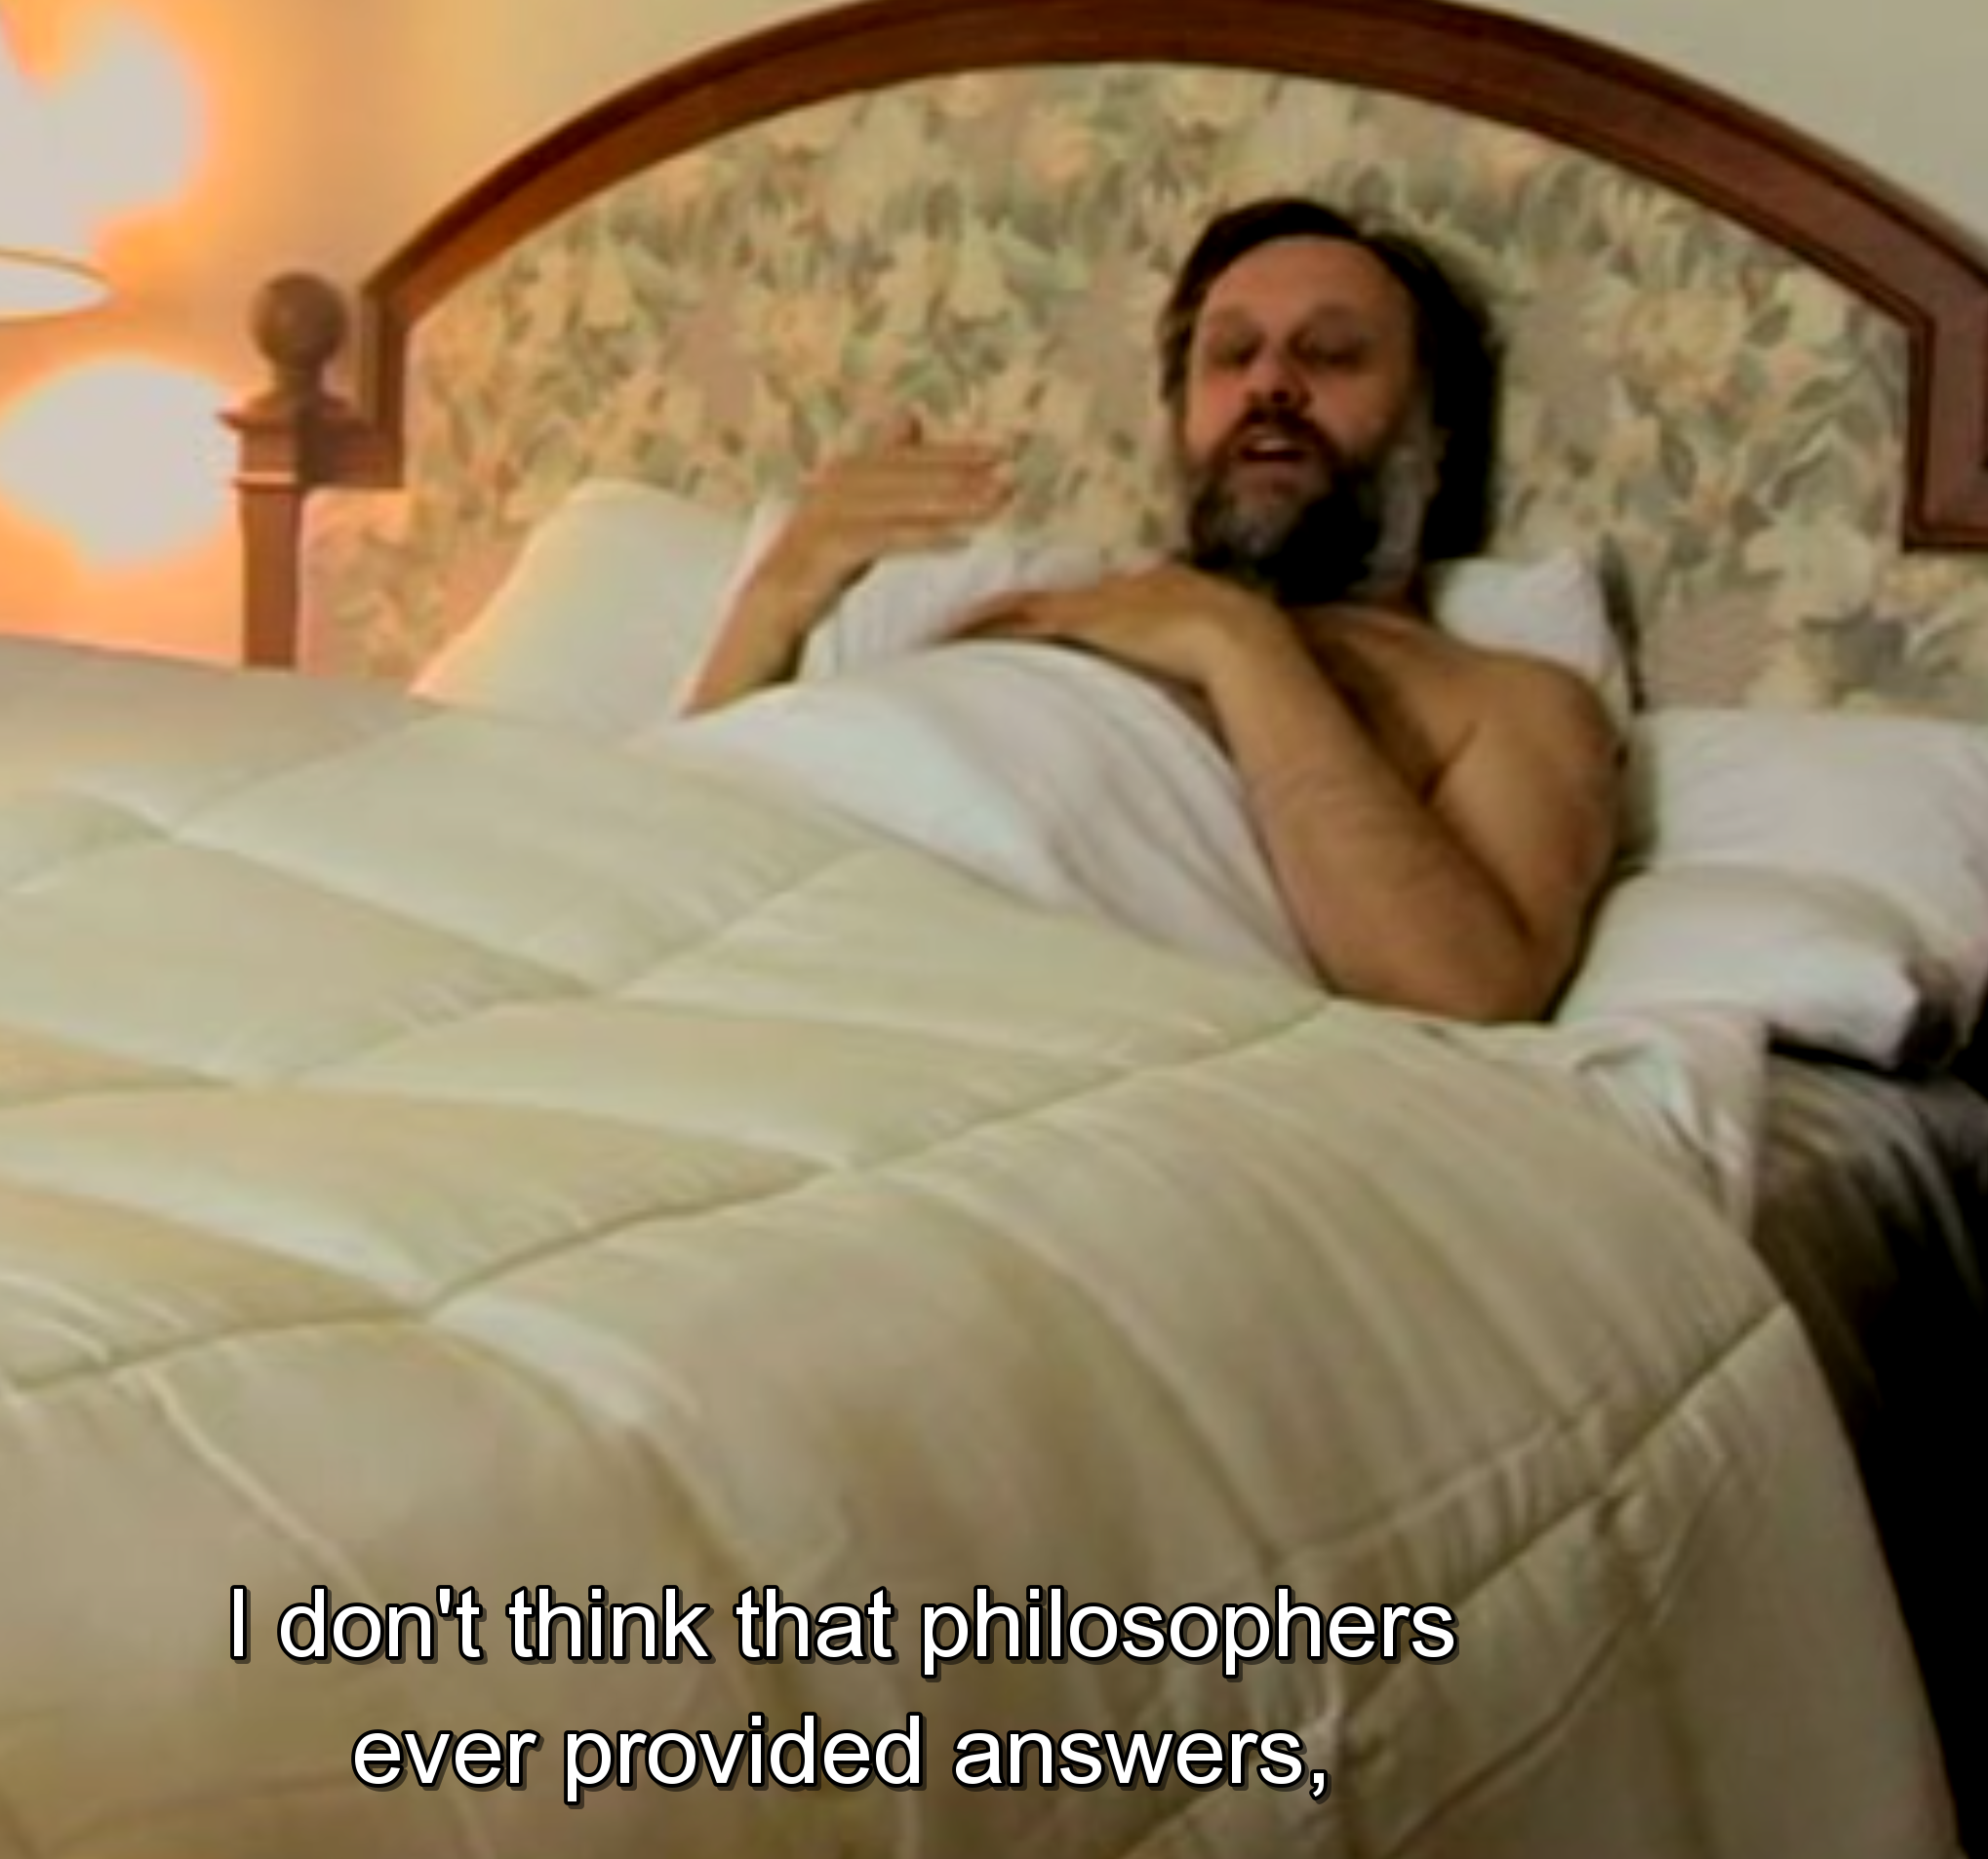
\includegraphics[width=0.5\textwidth]{images/template.png}
%	\caption{Template Bild}
%	\label{fig:template}
%\end{figure}

\end{document}
